\makeatletter
\let\my@xfloat\@xfloat
\makeatother
\documentclass[compressed,final,notitlepage,narroweqnarray,inline,twoside,]{ieee}

\makeatletter
\def\@xfloat#1[#2]{
\my@xfloat#1[#2]
\def\baselinestretch{1}
\@normalsize \normalsize
}
\makeatother
\usepackage{makeidx}
\usepackage{tikz}
\usepackage{graphicx}
\usepackage{caption}
\usepackage{subcaption}
\usepackage[caption=false]{subfig}
\usepackage{amsmath} 
\usepackage{amsfonts}
\usepackage{float}
\restylefloat{figure}
\usepackage[boxed]{algorithm2e}
\setlength{\parindent}{0cm}

\title[TITLE]{A Comparative Study Between Primallity Testing Algorithms.}
\author{By,Tamis van der Laan \& Author Samuel Austin }

\begin{document}
\maketitle

\begin{abstract}
In this paper we compare three one sided Monte Carlo primality testing algorithms, namely the Fermat’s, Miller-Rabin and Solovay-Strassen primality test algorithms and two deterministic primality testing algorithms, namely the Trial division algorithm and the Agrawal-Kayal-Saxena primality testing algorithms.  We will look at theoretical runtime complexity as well as practical run time complexity, Theoretical accuracy and practical accuracy. We will also look at the practicality of parallelizing the algorithms and look at their gain in runtime using our setup.
\end{abstract}
\section{Introduction}
\subsection{Fermat's Primality Test}
Fermat's primality test is quite simple. It makes use of fermat’s little theorem \cite{FLT} which is stated as followed:  
\begin{equation}
a^{p-1} \equiv  1 \mod p
\end{equation}
This theorem holds for any $1\leq a < p$ when $p$ is a prime number and a and integer. When a is composite at least half of the integer bases a will fail the test with the exception of so called Carmichael numbers. These Carmichael numbers will pass the test for most of the integer basses a. Although the test is flawed Carmichael numbers are rare and thus the test is still used in practical applications. This theorem is utilized in practice by generating $k$ random integer bases and testing if the theorem holds. If one fails the test the number is composite and if all pass the number is prime. The accuracy of the fermat primality test given that $n$ is not a Carmichael number is $2^{-k}$ where $k$ is the number of tests performed.
\begin{algorithm}[ht]
 \caption{Fermat's Primality Test}
 \KwIn{n,k}
 \KwOut{n is prime or composite}
 \For{$i \in \{1,...,k\}$}
 {
	$r \longleftarrow$ random(1,n-1) \;
	\If{$r^{n-1} \mod n \neq 1$}
	{
		\KwRet{Composite}\;
	}
 }
 \KwRet{Prime}\;
\end{algorithm}
\subsection{Solovay-Strassen Primality Test}
The Solovay Strassen primality test \cite{SS} is built upon the ideas of the original fermat’s primality test. The Solovay-Strassen primality test indeed takes a similar approach where instead of fermat’s little theorem the following theorem discovered by euler is used:
\begin{equation}
a^{(p-1)/2} \equiv \begin{pmatrix}\frac{a}{b}\end{pmatrix} \mod p
\end{equation}
Were (a/b) is called the jacobi symbol. This theorem will always hold for any base and prime number p. In contrast to the fermat primality test for any composite  number at least half of the integer bases pass the test stated above. The accuracy of the Solovay-Strassen primality test is therefore 2-k where k is the number of random bases tested. In principle the fermat’s primality test has the same accuracy but it suffers from the Carmichael numbers which are composite yet will pass the fermat’s little theorem for most bases (far more than half).  
\begin{algorithm}[ht]
 \caption{Solovay-Strassen Primality Test}
 \KwIn{n,k}
 \KwOut{n is prime or composite}
 \If{$n\neq 2 \wedge n \mod 2 = 0 \vee n<2$}
 {
 	\KwRet{Composite}\;
 }
 \For{$i \in \{1,...,k\}$}
 {
	$r \longleftarrow$ random(1,n-1) \;
	$jacobian \longleftarrow (n+jacobi(r,n)) \mod n$ \;
	$m \longleftarrow r^{(n-1)/2}$ \;
	\If{$jacobian=0 \vee m \neq jacobian$}
	{
		\KwRet{Composite}\;
	}
 }
 \KwRet{Prime}\;
\end{algorithm}
The run time complexity of the Solovay-Strassen Primality test is $O(k \cdot log^3 n)$. 
\subsection{Miller-Rabin Primality Test}
The Miller-Rabin test \cite{MR} is based on the Fermat test, just like the Solovay-Strassen test, but also includes elements of Euclid’s lemma.  Euclid’s lemma is based on the following:\\\\
if $x^2 \equiv 1 \mod p	$ then $(x-1)(x+1) \equiv 0 \mod p$\\\\
This means that prime $p$ can divide the product $(x-1)(x+1)$. Euclid’s lemma states that prime $p$ divides one of the factors $(x-1)$ or $(x+1)$. This implies that $x$ is congruent to $1 \mod p$ or $-1 \mod p$.\\\\ Based on this, the following must hold for any prime number $p>2$:\\
$p-1$ must be an even number and can be written as $2^s\cdot d$ where s and d are both positive and d is an odd number.\\\\
For each $a \in \{1,...,p-1\}$ one of the following must hold:\\\\
$a^d \equiv 1 \mod p \vee a^{2^rd} \equiv -1 \mod p$ were $r \in \{0,...,s-1\}$\\\\
The Miller-Rabin test then uses Fermat’s little theorem, $a^{p-1} \equiv 1 \mod p$, in combination with the above equalities in the following way:\\\\
If you keep taking square roots of $a^{n-1}$ and n is prime then you should end up with either $a^{2^rd} \equiv -1 \mod p$ with $r\in \{0,...,s-1\}$ or if all powers of 2 have been removed $a^d \equiv 1 \mod p$. \\\\
If neither of these cases are reached, $n$ must be composite, otherwise $n$ is probably prime.

\begin{algorithm}[ht]
 \caption{Miller-Rabin Primality Test}
 \KwIn{n,k}
 \KwOut{n is prime or composite}
 $s \longleftarrow n-1$ \;
 \While{$s \mod 2 = 0$}
 {
 	$s \longleftarrow \frac{s}{2}$\;
 }
 \For{$i \in \{1,...,k\}$}
 {
	$r \longleftarrow$ random(1,n-1) \;
	$t \longleftarrow s$\;
	$m \longleftarrow a^t \mod n$ \;
	 \While{$t \neq n-1 \wedge m\neq 1 \wedge m\neq n-1$}
	 {
	 	$m \longleftarrow m^2 \mod n$ \;
	 	$t \longleftarrow 2t$
	 }
	 \If{$m \neq n-1 \wedge t \mod 2 =0$}
	{
		\KwRet{Composite}\;
	}
 }
 \KwRet{Prime}\;
\end{algorithm}
The running time is $O(k\cdot log^3(n))$ and the accuracy of the test is equal to $4^{-k}$.


\subsection{Trial Division Primality Test}
Trial Division is the most trivial and straightforward deterministic primality test one can imagine. It simply exploits the fact that a prime number can only be divided with itself and 1. There is no need to test numbers beyond the square root of n and thus the worst case running time becomes $O(\sqrt{n})$.
\begin{algorithm}[ht]
 \caption{Trial Division Primality Test}
 \KwIn{n}
 \KwOut{n is prime or composite}

 \For{$i \in \{2,...,\sqrt{n}\}$}
 {
	 \If{$ n \mod i = 0$}
	{
		\KwRet{Composite}\;
	}
 }
 \KwRet{Prime}\;
\end{algorithm}
\subsection{Agrawal-Kayal-Saxena Primality Test}
\section{Accuracy Comparison}
Although the theoretical accuracies are known we tested the accuracy of the random algorithms in practice as they may deviate from the theoretical accuracy which are only upper bounds. Our first test will involve testing the first 500000 numbers for different number of tests k. We detect the errors by also running the deterministic Trial Division Primality Test. Under the assumption of the theoretic bounds we would expect to see 500000/2=250000 and 500000/4 =125000 errors when k=1. The histograms below show the results for k=1,2,3.
\begin{figure}[H]
        \centering
        \begin{subfigure}[b]{0.23\textwidth}
                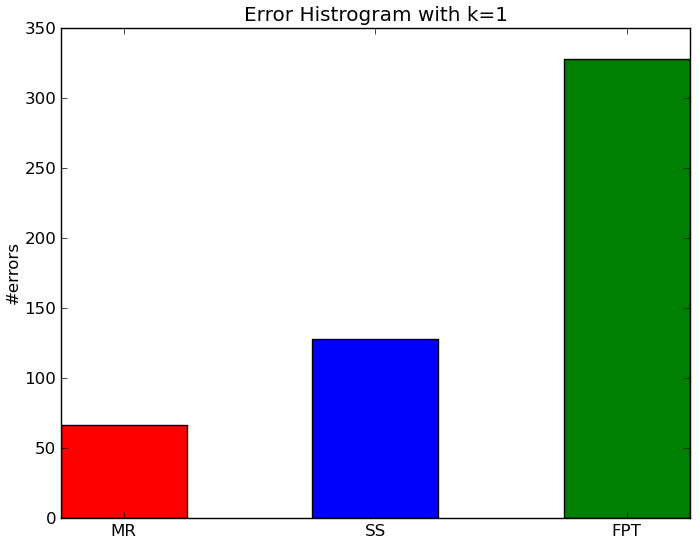
\includegraphics[width=\textwidth]{../images/Accuracy_k1}
                \label{fig:gull}
        \end{subfigure}%
        ~ 
        \begin{subfigure}[b]{0.23\textwidth}
                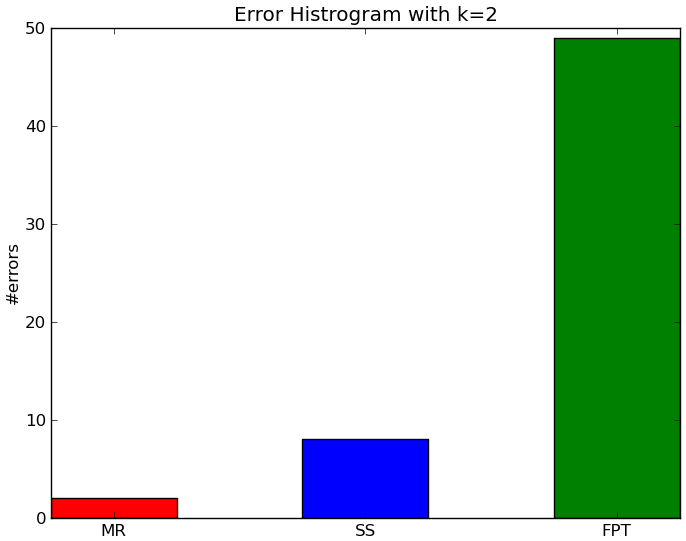
\includegraphics[width=\textwidth]{../images/Accuracy_k2}
                \label{fig:tiger}
        \end{subfigure}
        ~ 
        \begin{subfigure}[b]{0.23\textwidth}
                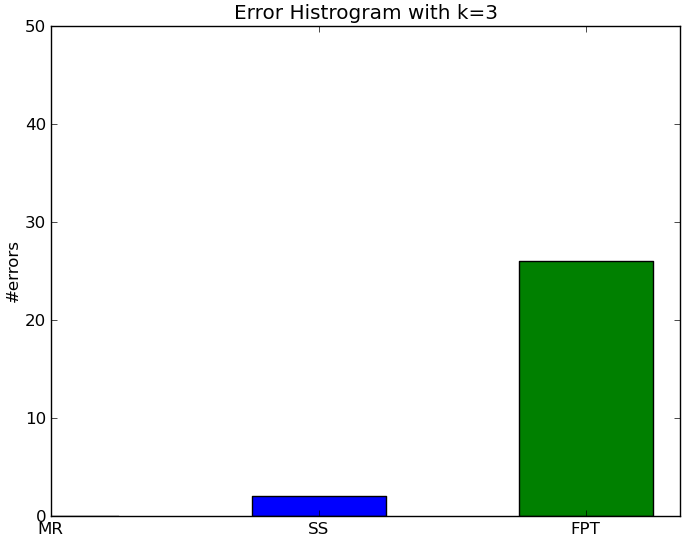
\includegraphics[width=\textwidth]{../images/Accuracy_k3}
                \label{fig:mouse}
        \end{subfigure}%
        ~ 
        \begin{subfigure}[b]{0.23\textwidth}
                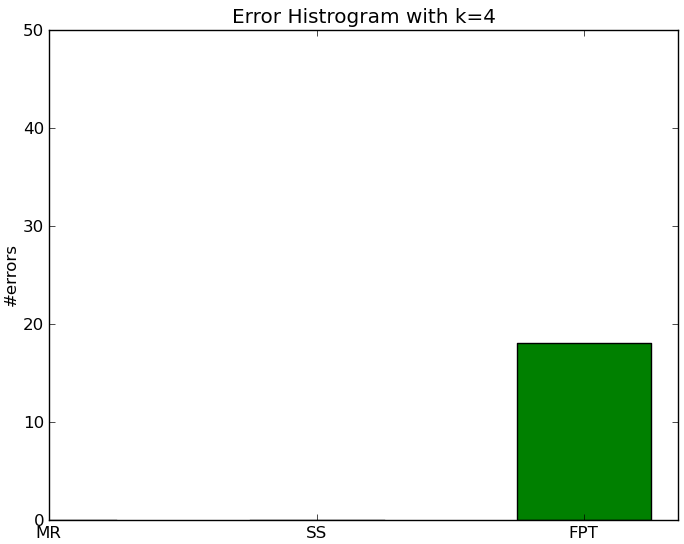
\includegraphics[width=\textwidth]{../images/Accuracy_k4}
                \label{fig:tiger}
        \end{subfigure}
        
        \caption{Pictures of animals}\label{fig:animals}
\end{figure}
We see that the algorithms perform significantly better than expected for k=1. Namely we make far viewer errors in practice than in theory. It is also clear that although the theoretical accuracy bounds of the Solovay-Strassen and the Fermat primality test are the same (except for the carmichael numbers) the Solovay-Strassen performs significantly better. We do see that the miller-rabin test is twice as accurate as the Solovay-Strassen test. This trend persists when k grows. The Fermat Primality Test  seems to half for k up to 3 but then gets stuck when k>3 most probably due to the remaining Carmichael numbers. This can also be seen from the shaky character in the plot below which illustrates the number of errors with increase of k.
\begin{figure}[H]
        \centering
        \begin{subfigure}[b]{0.45\textwidth}
                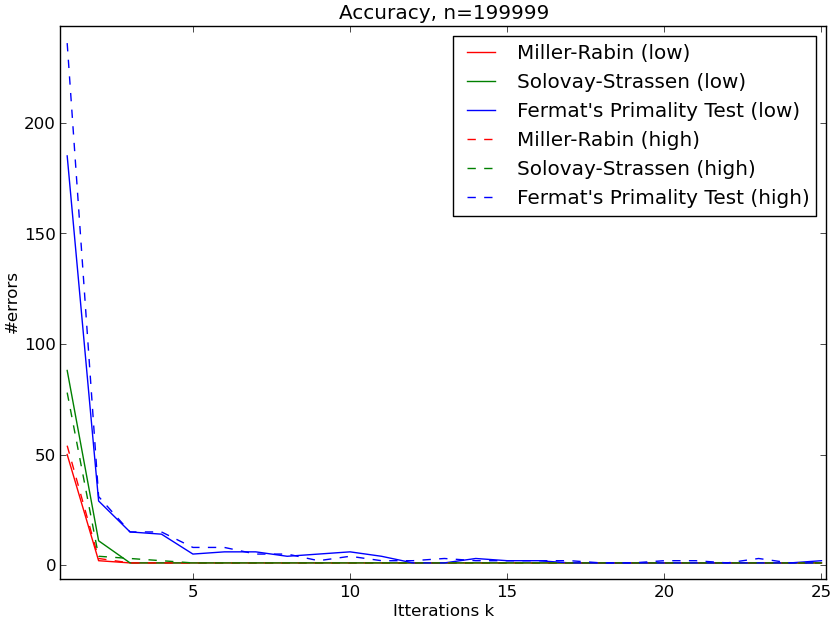
\includegraphics[width=\textwidth]{../images/Accuracy_all_exp}
                \label{fig:gull}
        \end{subfigure}
        \begin{subfigure}[b]{0.45\textwidth}
                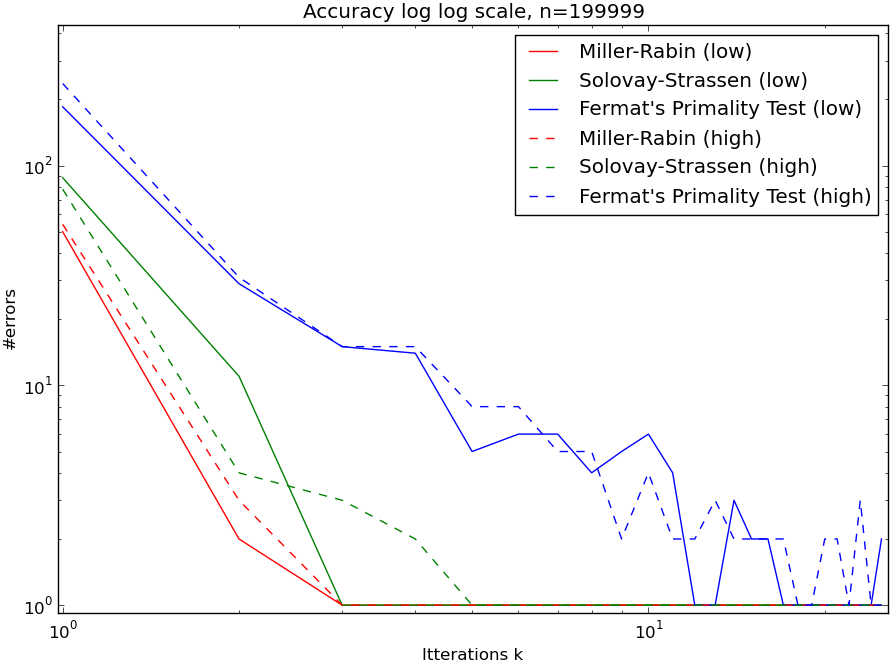
\includegraphics[width=\textwidth]{../images/Accuracy_all}
                \label{fig:tiger}
        \end{subfigure}
 
        \caption{Pictures of animals}\label{fig:animals}
\end{figure}
From the log log plot on the right we see that the Fermat Primality Test has a linear character in the beginning. But when k is increased further there error starts to shake and goes to zero further out then one would have expect when only looking at linear behavior at the beginning. This behavior stems from the Carmichael numbers who are persistent and require far more iterations to be correctly labeled as composite.\\\\ In theory the accuracy is independent of n, that is the magnitude of the number being tested. We tested this in practice by comparing accuracy in two different ranges, namely from 1 to 200000 and from 200000 to 400000, both results can be seen in the plot as a complete lines and striped lines respectively. We see that indeed small or large n numbers perform approximately the same. There is a small discrepancy but this is due to the fact that the density of primes decreases in the order of 1/log(n) (prime number theorem). 
\section{Run Time Comparisons}
We test the performance of both the Monte Carlo Algorithms as well as the Deterministic Algorithms both in a serial and parallel fashion. For this we used the following computing setup:
\begin{tabular}{l|l}
\hline
Processor & Intel Core i7-3630QM 2.4 GHz (8 cores)\\\hline
Memory: & 7.7 GB DDR3 \\\hline
OS: & Linux Mint 16 (Petra)\\\hline
\end{tabular}
The algorithms have been implemented in C++ and we use the Open Multi Processor library\cite{OMP} in order to parallelize our code. For modulo exponentiation we used the GNU Multiple Precision Library\cite{GMP} as these exponentiations easily get very large.
\subsection{Monte Carlo Primality Tests}
Next to the accuracy of the randomized primality tests, it is also useful to know the run time in order to determine which algorithm is most viable. For these tests we based the value k, the number of iterations run within each algorithm, on the theoretical accuracy of each primality test. As Miller-Rabin is twice as accurate compared to the other two we only run half the number of times.\\\\ As the speed of the randomized algorithms is quite high we used large numbers to generate the run time data. We used a range of 360000 numbers starting at 9999990074039999. For the first test we set the value k as 5 for the Miller-Rabin test and 10 for the others. Each primality test for each algorithm was run 5 times and the average run time was used to plot the graph.
\begin{figure}[H]
        \centering
        \begin{subfigure}[b]{0.5\textwidth}
                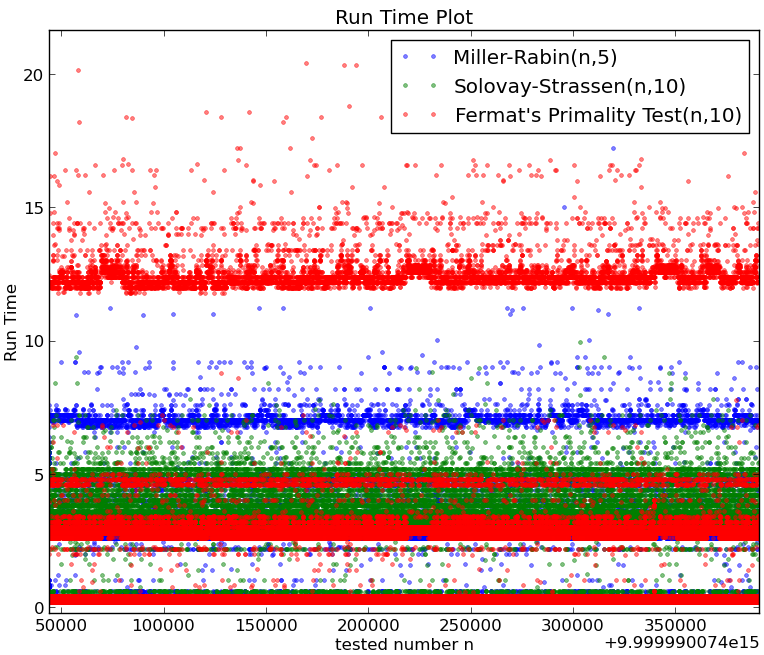
\includegraphics[width=\textwidth]{../images/all_singlethread_small_runtime}
                \label{fig:gull}
        \end{subfigure}
        \caption{Pictures of animals}\label{fig:animals}
\end{figure}
From the above graph we can see that the Fermat test is the slowest of the three randomized algorithms. The Solovay-Strassen test is the fastest, even though it runs twice the number of iterations compared to the Miller-Rabin test. 
\begin{figure}[H]
        \centering
        \begin{subfigure}[b]{0.5\textwidth}
                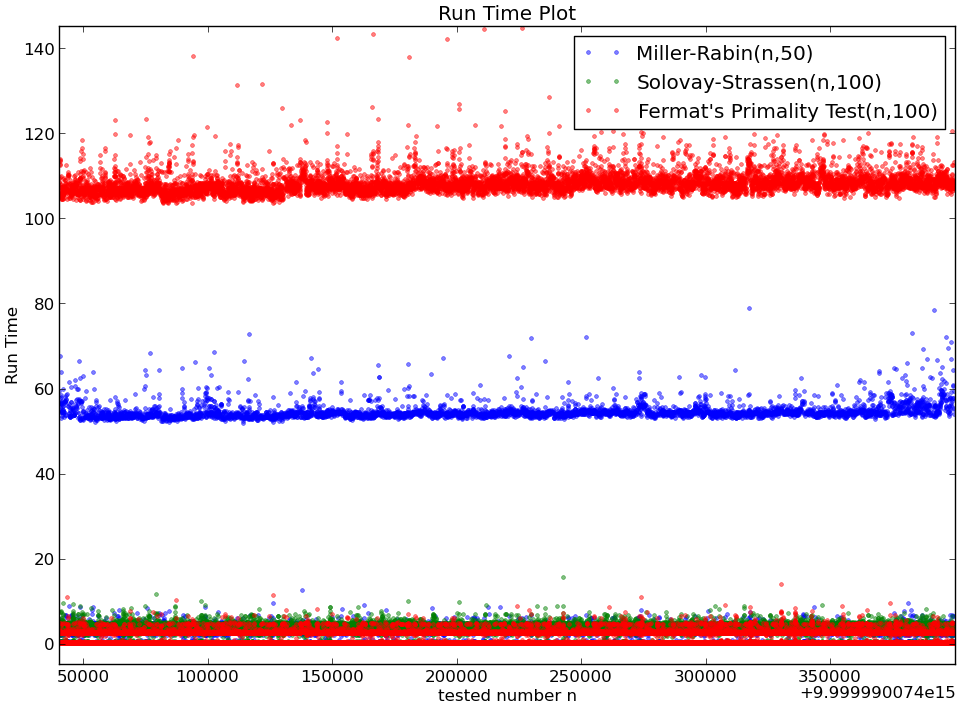
\includegraphics[width=\textwidth]{../images/all_singlethread_runtime}
                \label{fig:gull}
        \end{subfigure}
        \caption{Pictures of animals}\label{fig:animals}
\end{figure}
We also checked what the results would be if a large number of iterations was used. We set the Miller-Rabin test to do 50 iteration and the others to 100 iterations. From the graph we can see that the results are the same, but spread out further.\\\\ Based in the accuracy of the Miller-Rabin and Solovay-Strassen tests, there is no practical reason to use such a large number of iterations. However, the Solovay-Strassen is the fastest algorithm in both cases and therefore seems to be the most viable of the three.
\subsection{Deterministic Primality Tests}
\subsubsection{Trial Division Primality Test}
The first deterministic primality test we tested is the Trial Division Algorithm which has a theoretical runtime complexity of O(√n). We ran the algorithm from 1 up to 3000000 testing primality and recording the it’s runtime. The run time is an average of 5 independent runs in order to counteract cpu fluctuations which result in noise. The plotted results can seen below. 
\begin{figure}[H]
        \centering
        \begin{subfigure}[b]{0.5\textwidth}
                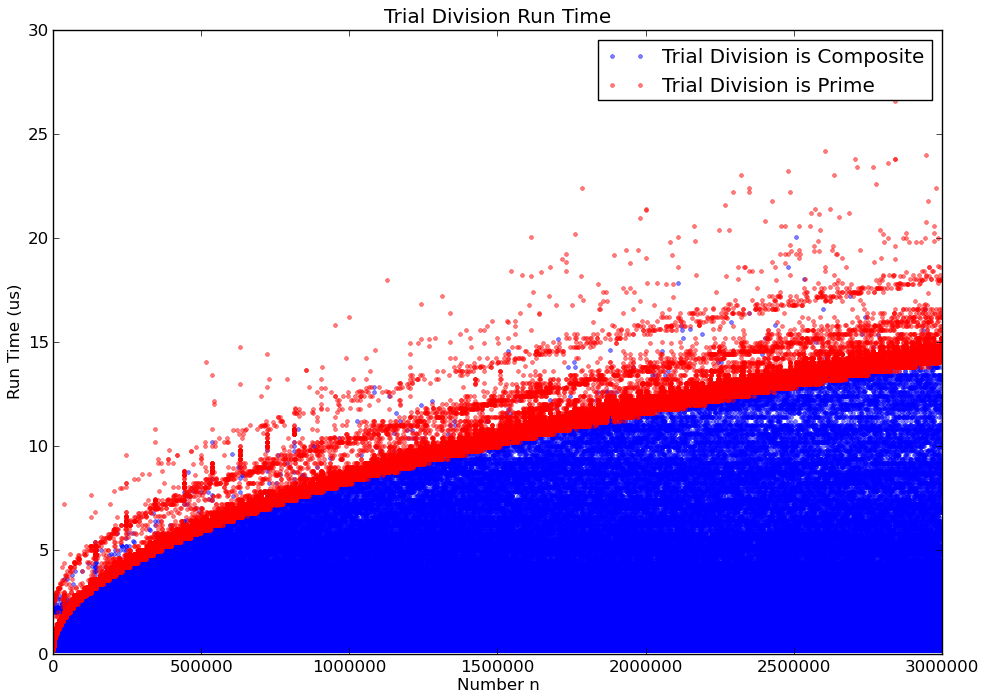
\includegraphics[width=\textwidth]{../images/isPrime}
                \label{fig:gull}
        \end{subfigure}
        \caption{Pictures of animals}\label{fig:animals}
\end{figure}
We clearly see the square root behavior in the plot closely reflecting the theoretical runtime complexity. The prime numbers are plotted in red while the composite numbers are plotted in blue. The prime numbers ride on top of the composite numbers as they form the worst case. The composite blue numbers seem to be approximately uniformly distributed between zero and the worst case.
\subsubsection{Agrawal-Kayal-Saxena Primality Test}
The second deterministic primality we tested was the Agrawal-Kayal-Saxena primality test. This test has a theoretic runtime complexity of O(). The plot below shows the practical run time of the primality test.
\begin{figure}[H]
        \centering
        \begin{subfigure}[b]{0.5\textwidth}
                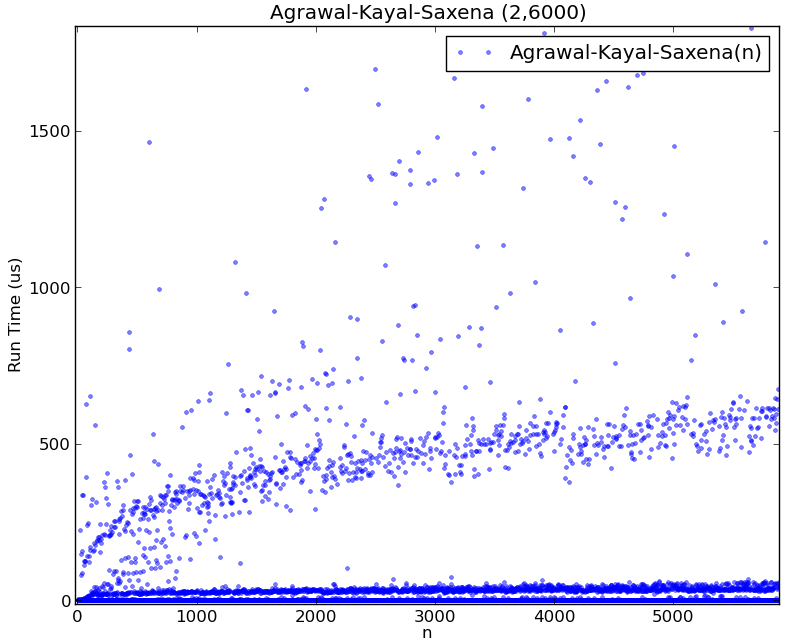
\includegraphics[width=\textwidth]{../images/AKS}
                \label{fig:gull}
        \end{subfigure}
        \caption{Pictures of animals}\label{fig:animals}
\end{figure}
We see that the plot splits into two parts, the lower part seems to consist of the composite and even numbers while the upper part consists of prime numbers. The upper part clearly shows the logarithmic behavior of the algorithm which is also present in the theoretical time complexity. For this plot we took an average of 10 runs to compute the run time for each number. We see that never the less outliers persist above the plot. 
\begin{figure}[H]
        \centering
        \begin{subfigure}[b]{0.5\textwidth}
                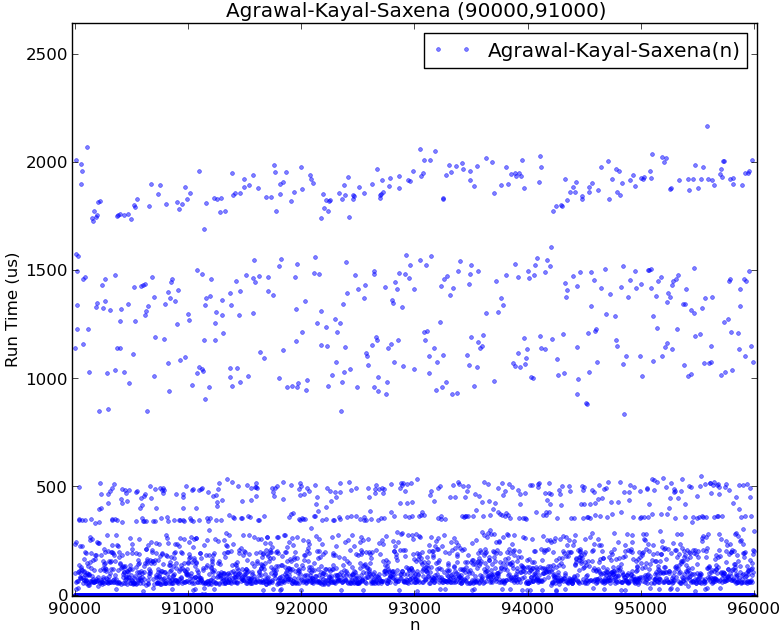
\includegraphics[width=\textwidth]{../images/AKS_large}
                \label{fig:gull}
        \end{subfigure}
        \caption{Pictures of animals}\label{fig:animals}
\end{figure}
\subsubsection{Trial Division vs Agrawal-Kayal-Saxena}
\section{Parallel Monte Carlo Primality Tests}
We experimented with the parallelization of the randomized algorithms to see if it would give any significant performance gain. For each algorithm we parallelized the iterations done within each algorithm as the operations within the iterations are independent of each other. For the measurements we used a range of numbers from 100000 to 120000. 
\subsubsection{Fermat}
\begin{figure}[H]
        \centering
        \begin{subfigure}[b]{0.5\textwidth}
                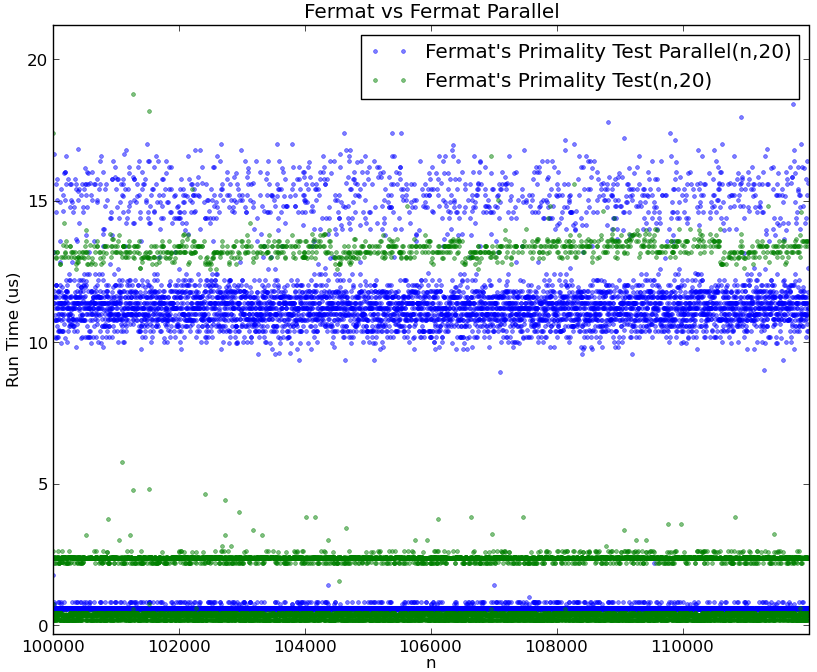
\includegraphics[width=\textwidth]{../images/FPT_FPTP_runtime}
                \label{fig:gull}
        \end{subfigure}
        \caption{Pictures of animals}\label{fig:animals}
\end{figure}
In the Fermat test, with the number of iteration set to 20, we can see that the difference in run time is quite insignificant. This is mainly due to the overhead of creating threads which doesn’t weigh up against the time gained by running the iterations in parallel. 
\begin{figure}[H]
        \centering
        \begin{subfigure}[b]{0.5\textwidth}
                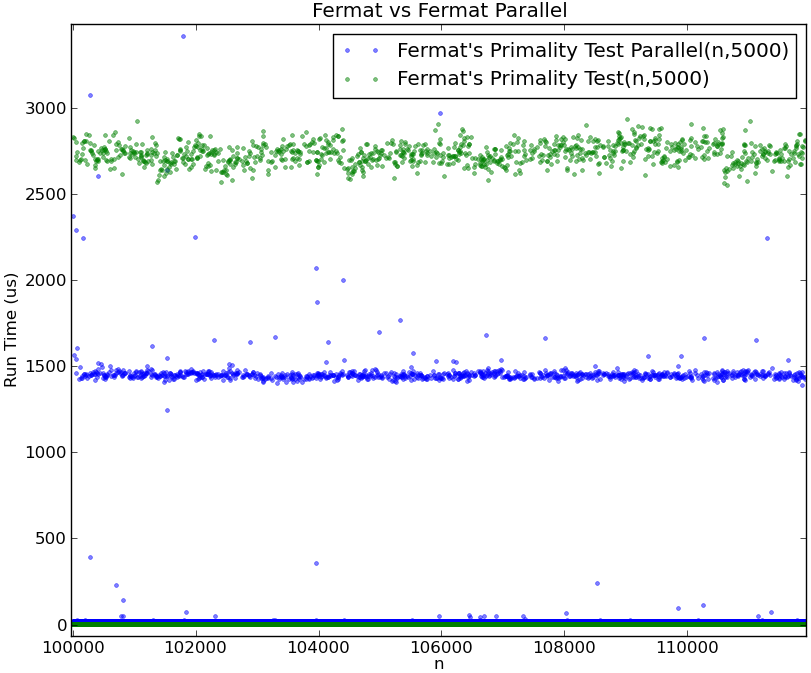
\includegraphics[width=\textwidth]{../images/FPT_FPTP_large_runtime}
                \label{fig:gull}
        \end{subfigure}
        \caption{Pictures of animals}\label{fig:animals}
\end{figure}
 In the above graph we can see that running the iterations in parallel only becomes advantageous when large values of k are used. In this case we set k to 5000.
\subsubsection{Miller-Rabin}
\begin{figure}[H]
        \centering
        \begin{subfigure}[b]{0.5\textwidth}
                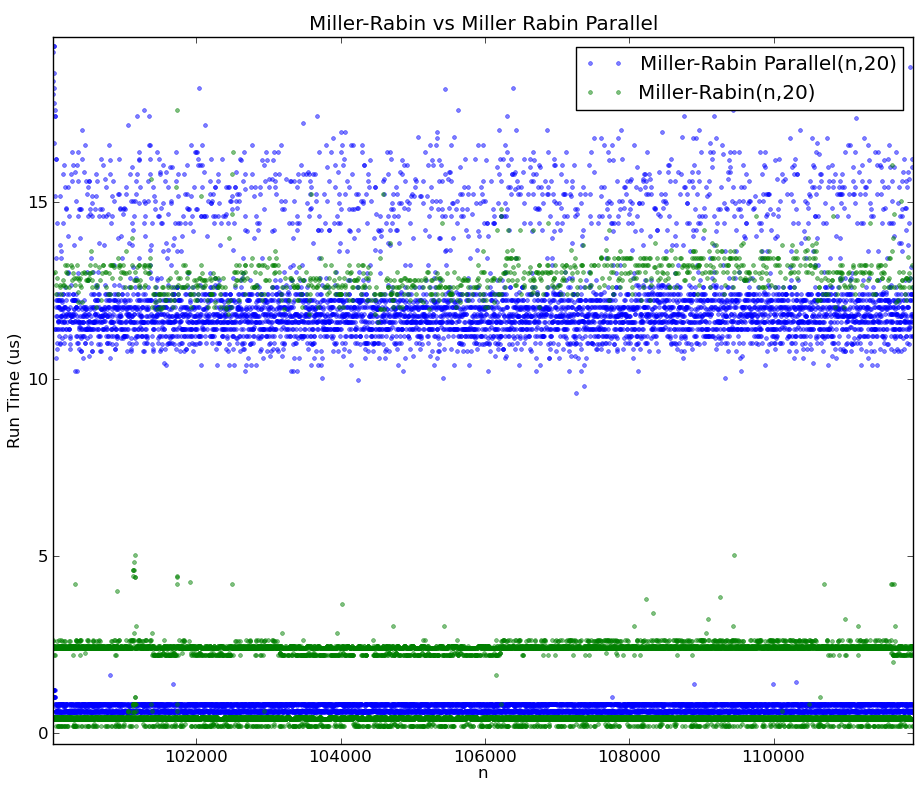
\includegraphics[width=\textwidth]{../images/MR_MRP_runtime}
                \label{fig:gull}
        \end{subfigure}
        \caption{Pictures of animals}\label{fig:animals}
\end{figure}
 The results for the Miller-Rabin test are similar to the Fermat test. With a low number of iterations the difference between a parallelized implementation and a regular implementation are negligible.
\begin{figure}[H]
        \centering
        \begin{subfigure}[b]{0.5\textwidth}
                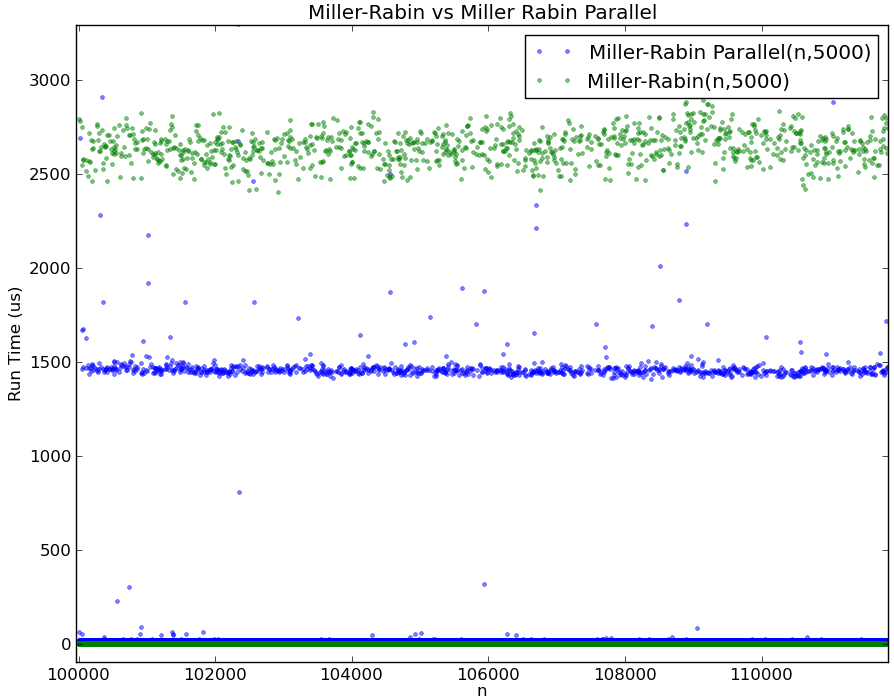
\includegraphics[width=\textwidth]{../images/MR_MRP_large_runtime}
                \label{fig:gull}
        \end{subfigure}
        \caption{Pictures of animals}\label{fig:animals}
\end{figure}
Running the Miller-Rabin test in parallel only becomes viable when using a high number of iterations.
\subsubsection{Solovay-Strassen}
\begin{figure}[H]
        \centering
        \begin{subfigure}[b]{0.5\textwidth}
                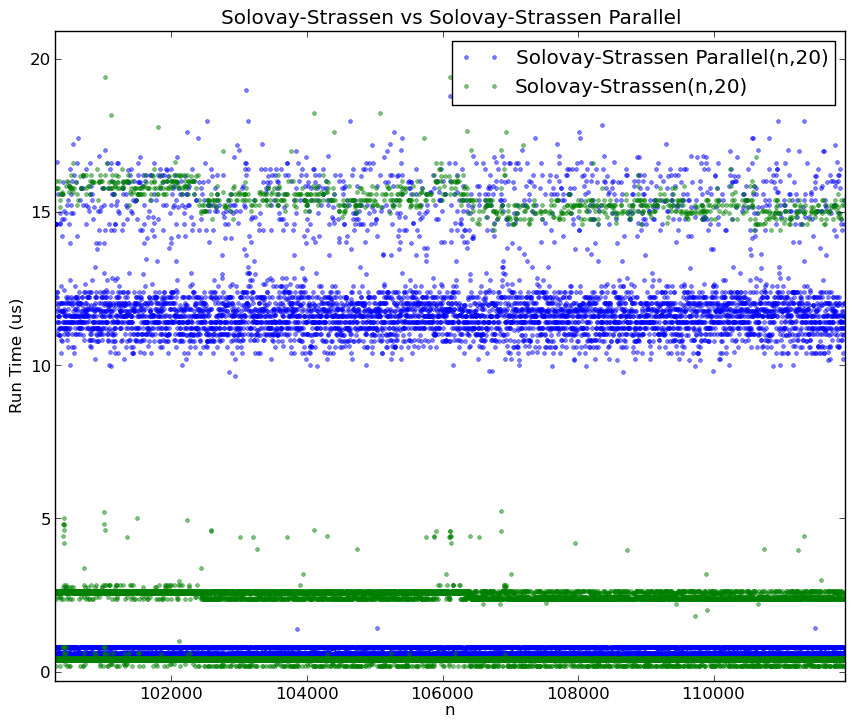
\includegraphics[width=\textwidth]{../images/SS_SSP_runtime}
                \label{fig:gull}
        \end{subfigure}
        \caption{Pictures of animals}\label{fig:animals}
\end{figure}
In the case of the Solovay-Strassen test we see that a parallel version does slightly better than the regular implementation.
\subsubsection{Solovay-Strassen}
\begin{figure}[H]
        \centering
        \begin{subfigure}[b]{0.5\textwidth}
                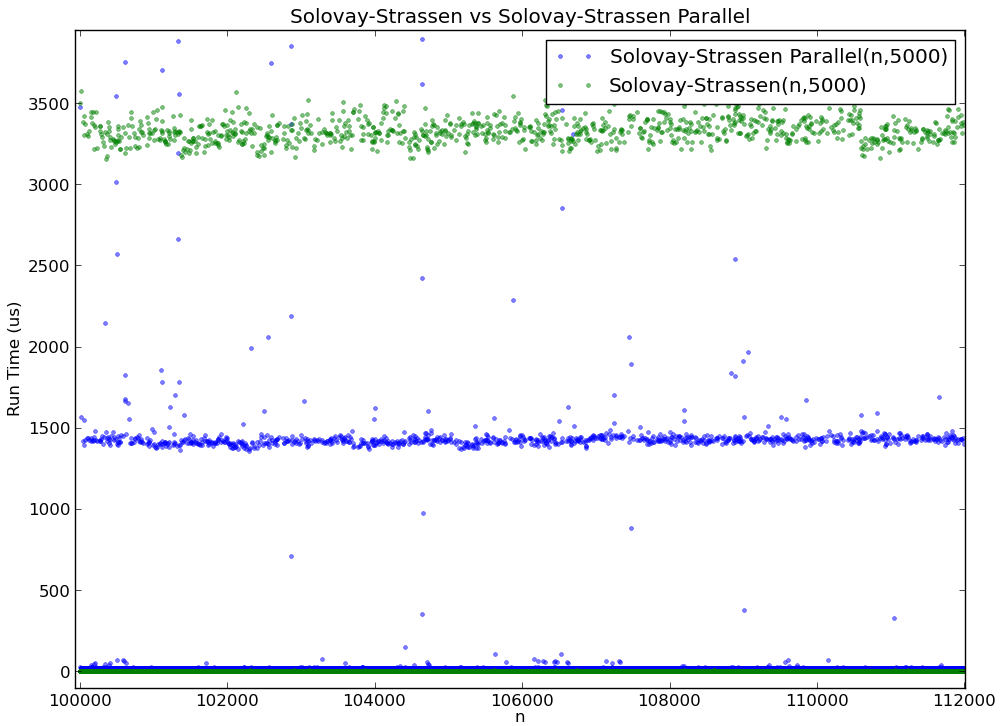
\includegraphics[width=\textwidth]{../images/SS_SSP_large_runtime}
                \label{fig:gull}
        \end{subfigure}
        \caption{Pictures of animals}\label{fig:animals}
\end{figure}
Once again, increasing the number of iteration causes a larger separation between the parallelized version and the regular implementation.
\subsubsection{Solovay-Strassen, Miller-Rabin and Fermat Parallel Comparison}
We also compared the parallel version of the three randomized algorithms to each other to see if parallelization would benefit one algorithm more than the other.
\begin{figure}[H]
        \centering
        \begin{subfigure}[b]{0.5\textwidth}
                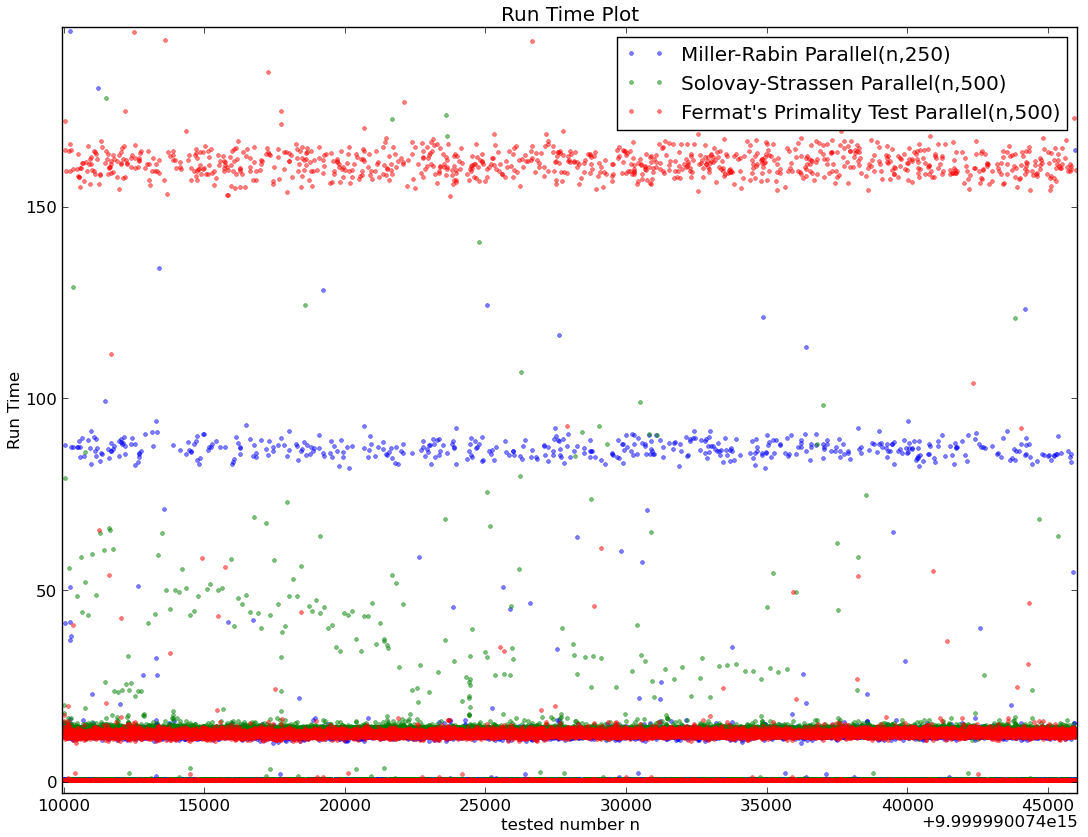
\includegraphics[width=\textwidth]{../images/compare_parallel_runtime}
                \label{fig:gull}
        \end{subfigure}
        \caption{Pictures of animals}\label{fig:animals}
\end{figure}
When comparing the parallel versions to each other we get the same results and the regular implementations. Solovay-Strassen is the fastest implementation, followed by Miller-Rabin, with Fermat coming last.
\subsubsection{Conclusion}
All in all, when using a relatively small number of iterations, the parallelized version does not give much of an advantage, if any. This is due to the overhead of creating threads and splitting up the work costing approximately the same amount of time as simply running the iteration in sequence.\\\\ When running the algorithms with a large number of iterations the parallel versions do give a significant advantage. However, the randomized algorithms they are generally not run with that many iterations as they already give very precise results with a relatively low number of iterations.
\section{Parallel Deterministic Primality Tests}
\subsection{Trial Division}
Parallelization was also applied to the trial division algorithm. We did two tests, one with small values for n (range of 0 to 10000) and one with large values (range of 10000 starting at $10^9$).
\begin{figure}[H]
        \centering
        \begin{subfigure}[b]{0.5\textwidth}
                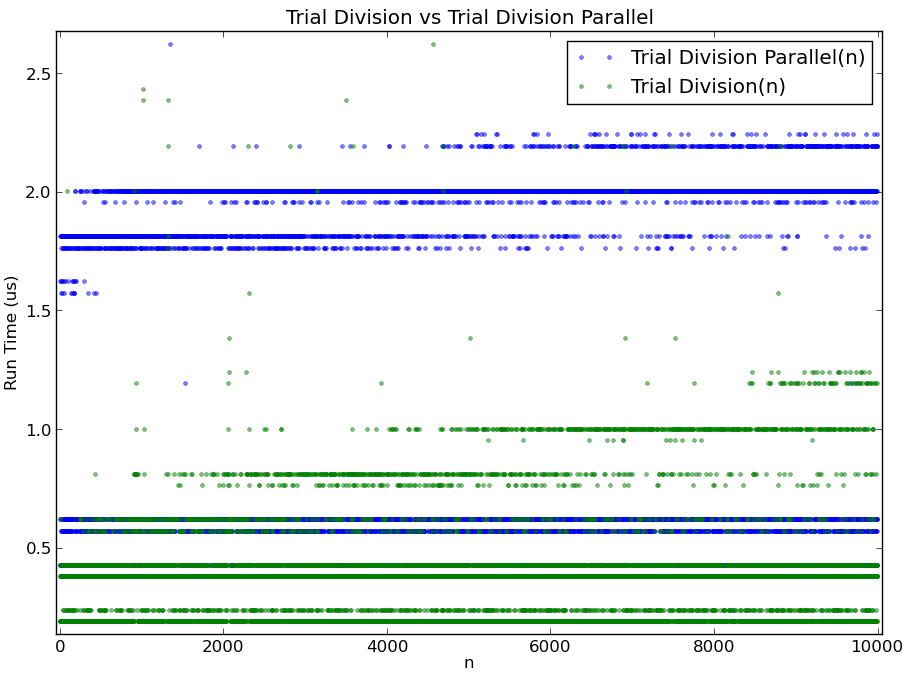
\includegraphics[width=\textwidth]{../images/isPrime_par_comparison_small}
                \label{fig:gull}
        \end{subfigure}
        \caption{Pictures of animals}\label{fig:animals}
\end{figure}
 When using small values of n we can see that, similarly to the randomized algorithms, the overhead of creating threads costs more time than calculating the answer in sequence. Due to the small size of the numbers and the speed of the algorithm, the boundaries of the precision of the measurement become visible but the difference in speed can still be distinguished.
\begin{figure}[H]
        \centering
        \begin{subfigure}[b]{0.5\textwidth}
                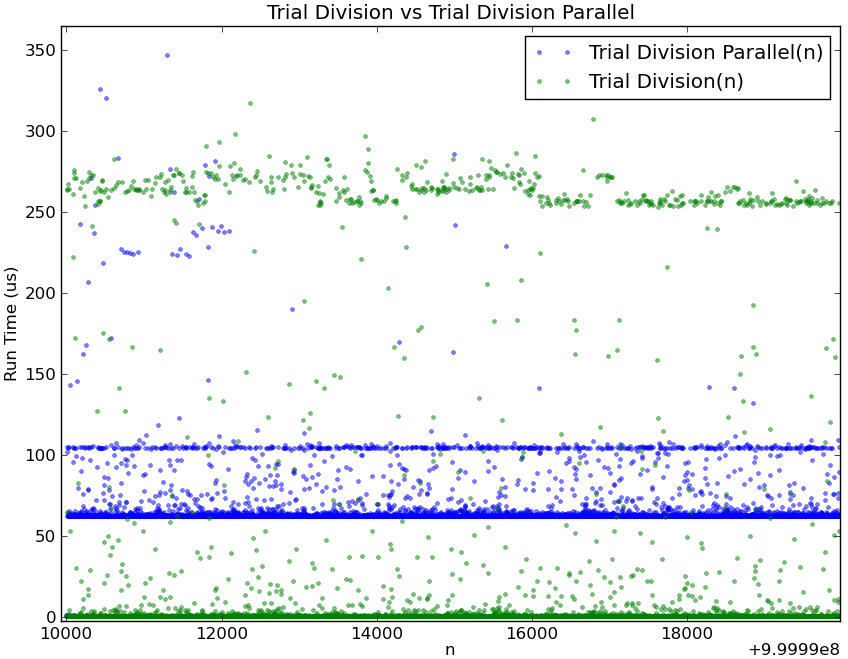
\includegraphics[width=\textwidth]{../images/isPrime_par_comparison}
                \label{fig:gull}
        \end{subfigure}
        \caption{Pictures of animals}\label{fig:animals}
\end{figure}
When using larger numbers we can see that the parallelized version has a great advantage over the original implementation. 
\subsubsection{Agrawal-Kayal-Saxena}
In the case of the Agrawal-Kayal-Saxena algorithm we were not able to parallelize it due to its complexity. It contains a number of loops with internal dependencies which means the iterations can not be run independently.
\section{The benefit of Randomization}
Randomization has clear benefits, although the deterministic primality tests are polynomial or even sub-polynomial in nature, for large prime numbers computation time becomes increasingly impractical. Random algorithms provide a arbitrary degree of accuracy with a constant amount of run time. This makes randomized in our opinion superior to the deterministic algorithms.
\begin{figure}[H]
        \centering
        \begin{subfigure}[b]{0.5\textwidth}
                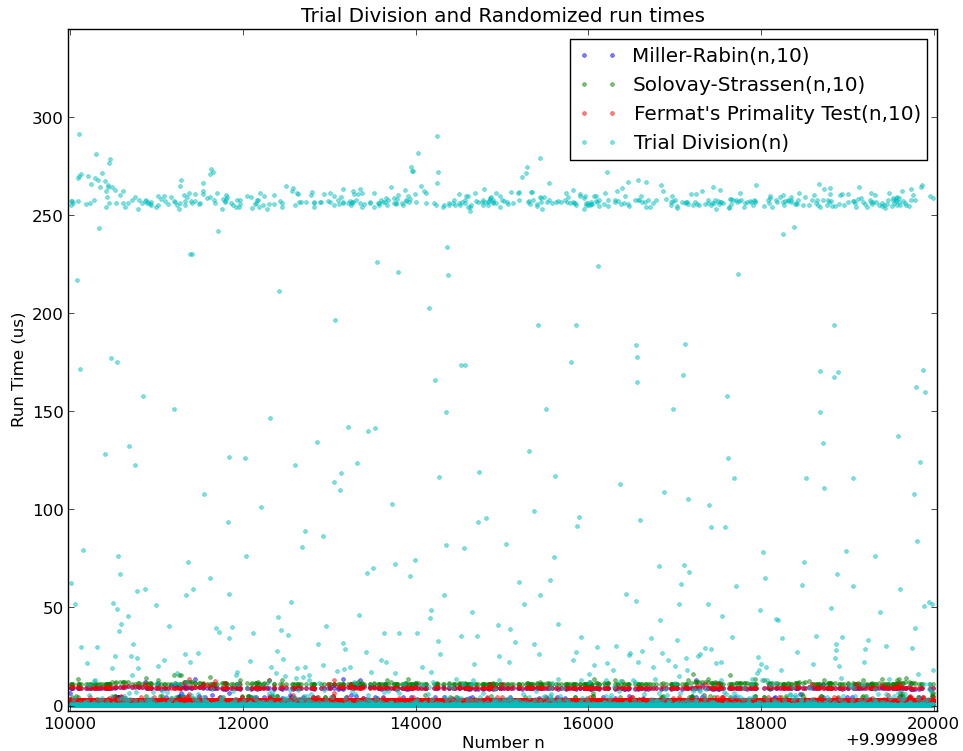
\includegraphics[width=\textwidth]{../images/isPrime_Randomized_runtime}
                \label{fig:gull}
        \end{subfigure}
        \caption{Pictures of animals}\label{fig:animals}
\end{figure}
In the above graph the randomized algorithms have been compared to the trial division algorithm on a range of 10000 numbers starting from $10^9$. As can be seen, the trial division algorithm is slower than the randomized algorithm by a large factor.\\\\ On top of the massive speed increase, the randomized algorithms also offer an impressive accuracy. Even at a low number of iterations, both the Miller-Rabin algorithm and the Solovay-Strassen algorithm make virtually no mistakes. The combination of high speed and high accuracy make the randomized algorithms very potent for finding prime numbers and generally a better choice than deterministic algorithms.
\bibliographystyle{plain}
\bibliography{mybib} 
\end{document}
